\title{Assignment 2: CS 215 \\ Solutions}
\author{
	Neeraj Dhake \\ 150050022
	\and
	Rohit Kumar Jena \\ 150050061
}
\date{20th August 2016}

\documentclass[11pt]{article}

\usepackage{amsmath}
\usepackage{amssymb}
\usepackage{float}
\usepackage{hyperref}
\usepackage{ulem}
\usepackage{flexisym}
\usepackage[margin=0.5in]{geometry}
% include graphics for images
\usepackage{graphicx}
\graphicspath{{../}}
% begin document
\begin{document}
\pagenumbering{gobble}
\maketitle
\newpage
\pagenumbering{arabic}

\textbf{Honor Code:} 
\begin{itemize}
\item We pledge by our honor that we will complete the assignments in a legitimate way and will not provide or recieve any unauthorized help. 
\end{itemize}
\vspace{5mm}
\textbf{Instructions to run code: }
\begin{itemize}
	\item{
		The folder `code' contains all the code written for the assignment. Here is how we run them. From the MATLAB command line, simply typing \textit{partA},\textit{partB},\textit{partC} will run the programs given in Question 7. 
	} 
	\item {
		The file \textit{frequencyCalc.m} calculates the values of $p_{X_1}(x1)$, $p_{X_2}(x2)$ and $p_{X_1X_2}(x_1,x_2)$. The inputs required are the two matrices $X_1,X_2$.
	}
	\item{
		The file \textit{corCoeff.m},\textit{qmi.m}, and \textit{anotherMeasure.m} give the values of Correlation Coefficient, QMI and the custom value. The code is commented so it can understood easily. 
		To be on the safe side, we have written the code for Correlation Coefficient rather than using the default routine.
	}
\end{itemize}
% \\
% \\
\textbf{Solutions: }
% solutions begin here
\begin{enumerate}
	
	\item{
		% Question 1
		There are 2 random variables $X$ and $Y$ having pdf $f_X(x)$ and $f_Y(y)$ and joint pdf $f_{XY}(x,y)$.

		To find the cdf and pdf of random variable $Z=XY$, we take $P(Z\leq a)$.

		$$ P(Z \leq a) = P(XY \leq a) $$
		$$ P(XY \leq a) = \int{\int_{A}{f_{XY}(x,y)\cdot dx\cdot dy}} $$
		Since the function $xy=a$ has discontinuity at $x=0$, we have to write two terms, one from $(-\infty,0)$ and another from $(0,\infty)$ such that,
		
		$$ F_Z(a) = P(Z \leq a) = \int_{x=-\infty}^{x=0}{\int_{y=\frac{a}{x}}^{y=\infty}{f_{XY}(x,y)\cdot dy\cdot dx}} + \int^{x=\infty}_{x=0}{\int^{y=\frac{a}{x}}_{y=-\infty}{f_{XY}(x,y)\cdot dy\cdot dx}} $$

		To find the pdf, we simply differentiate w.r.t. $a$ to get,
		$$ f_Z(a) = \int_{x=-\infty}^{x=0}{-\frac{1}{x}\cdot{f_{XY}(x,\frac{a}{x})\cdot dx}} + \int^{x=\infty}_{x=0}{\frac{1}{x}\cdot{f_{XY}(x,\frac{a}{x})\cdot dy\cdot dx}} $$

		Similarly, for $P(X \leq Y)$, we take $X \geq x$ and find $Y \geq X$, hence, we can write in terms of joint probability,

		$$P(X \leq Y) = \int_{y=x}^{y=\infty}{\int_{x=-\infty}^{x=x}{f_{XY}(x,y)\cdot dx\cdot dy}} $$ \\

		To find the pdf, we differentiate w.r.t. $a$ to get,
		$$ p_{XY}(X\geq y) = $$

		% Now for independent variables.
		For independent variables, we can substitute $f_{XY}(x,y) = f_X(x)\cdot f_Y(y) $
		$$ F_Z(a) = P(Z \leq a) = \int_{x=-\infty}^{x=0}{\int_{y=\frac{a}{x}}^{y=\infty}{(f_Y(y)\cdot dy)\cdot f_X(x)\cdot  dx}} + \int^{x=\infty}_{x=0}{\int^{y=\frac{a}{x}}_{y=-\infty}{(f_Y(y)\cdot dy)\cdot f_X(x)\cdot  dx}} $$

		Integrating w.r.t. $y$ first, we get,
		$$\implies F_Z(a) = \int_{x=-\infty}^{x=0}{ \Bigg(1-F_Y\Bigg(\frac{a}{x}\Bigg)\Bigg)\cdot f_X(x)\cdot  dx} + \int^{x=\infty}_{x=0}{F_Y\Bigg(\frac{a}{x}\Bigg)\cdot f_X(x)\cdot dx}$$


		$$\implies F_Z(a) = F_X(0) + \int^{x=\infty}_{x=0}{F_Y\Bigg(\frac{a}{x}\Bigg)\cdot f_X(x)\cdot dx} - \int_{x=-\infty}^{x=0}{F_Y\Bigg(\frac{a}{x}\Bigg)\cdot f_X(x)\cdot  dx}$$

		For the case $X \leq Y$, substitute $f_{XY}(x,y) = f_X(x)\cdot f_Y(y) $ to get,
		$$ P(X \leq Y) = \int_{y=x}^{y=\infty}{\int_{x=-\infty}^{x=x}{f_X(x)\cdot f_Y(y)\cdot dx\cdot dy}}  $$

		$$ \implies P(X \leq Y) = \int_{x}^{\infty}{f_Y(y)\cdot dy}\cdot \int_{-\infty}^{x}{f_X(x)\cdot dx} $$

		$$ \implies P(X \leq Y) = \int_{-\infty}^{\infty}{f_X(x)\cdot(1-F_Y(x))\cdot dx} $$

		Integrating w.r.t. $x$ , we get the final expression.
		$$ \therefore P(X \leq Y) = 1 - E[F_Y(x)] $$

	}

	\item{
		$X_1, X_2 .... X_n$ are $n$ I.I.D. random variables. \\
		Now, $Y_1 = max(X_1, X_2 .... X_n) $. To provide the CDF of $Y_1$, we need to find the probablity that $Y_1$ is less than $a$. \\

		So, now if we conduct an experiment to determine the value of the random variable $X$ $n$ times, $Y_1$ will be less than $a$ only if $X_i \leq a$, $ \forall{i} $. \\

		\begin{center}
			$P(Y_1 \leq a) = P(X_1 \leq a) $ and $ P(X_2 \leq a)$ .... and $P(X_n \leq a)$
		\end{center}
		Since $X$ is an I.I.D. random variable, we can simply multiply the probabilities of the right hand side since the result of one experiment doesnot affect the result of the other, we have, \\
		$$P(Y_1 \leq a) = P(X_1 \leq a)*P(X_2 \leq a) ... *P(X_n \leq a)$$
		\begin{center}
			$P(Y_1 \leq a) = F_X{(a)}*F_X{(a)} ... *F_X{(a)}$  (n times) \\
		\end{center}
		$$P(Y_1 \leq a) = {(F_X(a))}^n$$
		\\
		Hence, $$F_{Y_1}(a) = (F_{X}(a))^n$$	\hfill{... (cdf of $Y_1$)} \\
		Differentiating w.r.t. a, we get, \\ \\
		$$F^{'}_{Y_1}(a) = f_{Y_1}(a) = \frac{\mathrm{d}(F_{X}(a))^n }{\mathrm{d} a}  = n\cdot (F_{X}(a))^{n-1}\cdot f_X(a)$$\\
		$$f_{Y_1}(a) = n\cdot (F_{X}(a))^{n-1}\cdot f_X(a)$$ \hfill{... (pdf of $Y_1$)} 
		% Now for Y_2

		Now, $Y_2 = min(X_1,X_2,..X_n)$ \\

		So, now if we conduct an experiment to determine the value of the random variable $X$ $n$ times, $Y_2$ will be \textbf{more} than $a$ only if $X_i \geq a$, $ \forall{i} $. \\ \\

		\begin{center}
			$P(Y_2 \geq a) = P(X_1 \geq a) $ and $ P(X_2 \geq a)$ .... and $P(X_n \geq a)$
		\end{center}

		Since $X$ is an I.I.D. random variable, we can simply multiply the probabilities of the right hand side since the result of one experiment doesnot affect the result of the other, we have, \\

		$$\implies P(Y_2 \geq a) = P(X_1 \geq a)*P(X_2 \geq a) ... *P(X_n \geq a)$$
		$$\implies P(Y_2 \geq a) = (1-P(X_1 \leq a))*(1-P(X_2 \leq a)) ... *(1-P(X_n \leq a))$$
		$$\implies P(Y_2 \geq a) = (1-F_X{(a)})*(1-F_X{(a)}) ... * (1-F_X{(a)})$$ \hfill{... (n times)} \\
		$$\implies P(Y_2 \geq a) = (1-{(F_X(a))})^n$$
		$$\implies 1- F_{Y_2}(a) = (1-{(F_X(a))})^n$$
		$$F_{Y_2}(a) = 1 - (1-{(F_X(a))})^n $$ \hfill{... (cdf of $Y_2$)} \\
		\\Differentiating w.r.t. a, we get, \\ \\
		$$f_{Y_2}(a) = n\cdot (1-F_{X}(a))^{n-1}\cdot f_X(a)$$ \hfill{... (pdf of $Y_1$)} \\
	}

	\item{
	Question 3
	}	

	\item{
		Let $X$ and $Y$ be two random independent random variables. For them, we have the following relation,
		$$f_{X,Y}(x,y) = f_X(x)\cdot f_Y(y)$$
		$$\implies E(XY) = E(X)\cdot E(Y)  $$

		Now, we define covariance of $X$, $Y$ as, 
		$$ cov(X,Y) = E[(X-\mu_X)\cdot(Y-\mu_y)] $$
		$$ = E[XY - \mu_xY - \mu_yX + \mu_x\mu_y]$$
		Using linearity of the expectation value operator, we get,
		$$ = E[XY] - E[\mu_xY] - E[\mu_yX] + E[\mu_x\mu_y]$$
		$$ = E[XY] - \mu_x\mu_y - \mu_x\mu_y + \mu_x\mu_y$$
		$$ = E[XY] - E[X]\cdot E[Y] $$
		Now since $E[XY] = E[X]\cdot E[Y]$, we have,
		$$cov(X,Y) = 0 $$

		For the converse, we take the following two random variables,
		\[X =  \begin{cases} 
		      1 &  ,P(X=1) = 0.5 \\
		      -1 &  ,P(X=-1) = 0.5\\
		   \end{cases}
		\]
		and
		\[Y =  \begin{cases} 
		      0.5 & ,X=1 \implies P(Y=0.5)=0.5 \\
		      -0.5 & ,X=1 \implies P(Y=-0.5)=0.5  \\
		      0 & ,X = -1 \implies Y=0 \\
		   \end{cases}
		\]

		These two random variables are obviously dependent, since if $X=0$, we can determine $Y$, and similarly for $X=1$.
		The covariance of these two variables will be ,
		$$cov(X,Y) = \frac{ \sum{(X-\mu_x)(Y-\mu_y)}}{(N-1)\sigma_x\sigma_y} = E[XY]-E[X]\cdot E[Y] $$
		Now, we have $E[X] = E[Y] = 0$, since the probability of $X$ taking any value is equal, and same for $Y$. Since all the values are centered around 0, we can say the statement without calculating it. We can calculate the value very easily as well. 
		$$\implies cov(X,Y) = E[XY] $$
		Now,
		$$ E[XY] = 1*0.5 + 1*-0.5 + -1*0  = 0 $$
		$$ \implies cov(X,Y) = E[XY] - E[X]\cdot E[Y] = 0-0\cdot0 = 0$$
		\begin{center}
			$\therefore$ , $X$ and $Y$ are dependent but have 0 covariance.
		\end{center}
	}

	\item{
		Question 5
	}

	\item{
		A function $g(x)$ is a convex function.
		Let $X$ be a random variable with $E[X]=\mu$. 
		Now, let $l(x)$ be the equation of the tangent at $x=\mu$.
		$$\implies l(x) = g\textprime(\mu)\cdot(x-\mu) + g(\mu)$$

		Now, we have $g(x) \geq l(x) ,\forall x \in \mathbb{R} $, we can write, 
		$$\int_{-\infty}^{\infty}{g(x)\cdot f_X{x}\cdot dx} \geq \int_{-\infty}^{\infty}{l(x)\cdot f_X{x}\cdot dx} $$
		$$\implies E[g(X)] \geq E[l(X)]$$
		Substitute $l(X) = g\textprime(\mu)\cdot(X-\mu) + g(\mu)$ to get ,
		$$E[l(X)] = E[g\textprime(\mu)\cdot(X-\mu) + g(\mu)]$$
		$$ = g\textprime(\mu)\cdot(E[X]-\mu) + g(\mu)$$
		$$ = l(E[X]) = l(\mu)$$
		Now, at $x=\mu, l(x) = g(x)$,so we get,
		$$E[l(X)] = l(E[X]) = g(E[X]) $$
		$$ \therefore E[g(X)] \geq g(E[X]) $$
	}

	\item{
		(a) Values computed with unaltered image - \\ \\
		\textbf{Correlation Coefficient} = 0.9841 \\
		\textbf{QMI} = 3.9643 \\
		\textbf{Another measure} = 51.5729

		(b) The code and instructions are provided. The graph is given below.
		\begin{figure}[H]
		\caption{Correlation Coefficient v/s z}
		\centering
		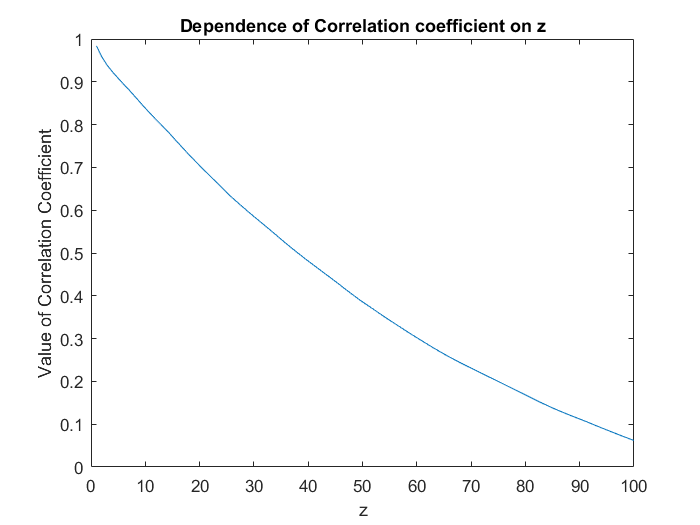
\includegraphics[width=\textwidth]{partB}
		\end{figure}
		
		(c) After scrambling the values, we ran the program another time and got the following results - \\ \\
		\textbf{Correlation Coefficient} = -0.0293 \\
		\textbf{QMI} = 3.8319 \\
		\textbf{Another measure} = 50.8610 \\ \\ 
		Original values (when image wasn't scrambled) - given in (a)


		}
\end{enumerate}

\end{document}